\section{Architektur des Microservice}
\label{sec: Architektur des Microservice}
Der Microservice Warenwirtschaft wurde in der Programmiersprache Go\footnote{https:\//golang.org\/doc\/} entwickelt.
Go-Anwendungen bestehen aus Packages, in denen die einzelnen Go-Files organisiert sind.
Ohne Klassen zu besitzen ist Go objektorientiert, es besitzt Struct und Interface, die auch vererbt werden könne.
Des Weiteren wird durch Groß-/Kleinschreibung definiert, ob die Methode auch außerhalb des Struct oder Packages verwendet werden kann.
Die Warenwirtschaft setzt sich aus den neun Packages zusammen, die die Abbildung \ref{pic:Struktur des Microservice} darstellt. In den nachfolgenden Unterkapiteln \ref{subsec: Presentation Layer} und \ref{subsec: Application Layer} werden die Packages und die darin enthaltenen Go-Files des Presentation sowie des Application Layers kurz vorgestellt. \par
Go-Files mit der Bezeichnung \texttt{<<Name>>\_test.go} beinhalten Whitebox-Testfälle um die Funktionen der benannten Go-Files zu prüfen. Aus Gründen der Übersichtlichkeit werden diese Files hier nicht explizit aufgeführt. Die Weiteren Unterkapitel beschreiben die Schnittstellen, den Persistant Layer sowie das Admin-Frontend und schließlich die Anpassung des Monolithen, um den Microservice Warenwirtschaft in diesen zu integrieren.

\begin{figure}[H]
	\centering
	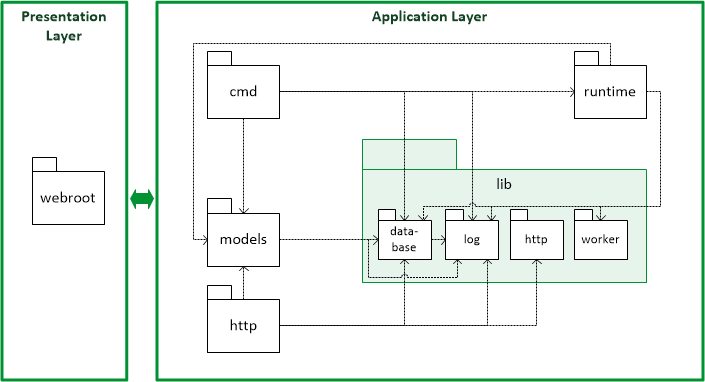
\includegraphics[width=0.95 \textwidth]{./pics/struktur.png}
	\caption{Paketdiagramm des Microservice}
	\label{pic:Struktur des Microservice}
\end{figure}

\newpage
\subsection{Schnittstellen zu anderen Microservices}
\label{subsec: Schnittstellen zu anderen Microservices}
Der Microservice Warenwirtschaft weißt drei Schnittstellen\footnote{Da es nicht Teil der übergeordneten Aufgabenstellung war, die Microservices der einzelnen Projektgruppen zu einem lauffähigen Webshop zusammenzufügen, greift die Warenwirtschaft an diesen Stellen auf Testdaten zurück} zu anderen Microservices auf. Zunächst greift der Microservice Warenwirtschaft für die Authentifizierung der Benutzer des Admin-Frontends vollständig auf einen Microservice Benutzerauthentifizierung zurück. Anstelle einer Login-Maske weißt das Admin-Frontend deshalb nur einen Icon in Form eines Schlosses auf. Dieser symbolisiert, ob ein Benutzer die passende Berechtigung für das Admin-Front besitzt (Schloss geschlossen) oder nicht (Schloss geöffnet).
Durch diesen Icon wird ein Session-Token gesetzt, welcher durch den gemocked Authentifizierten Microservice die benötigten Berechtigungen erlaubt.\par
Weiter benötigt der Microservice Warenwirtschaft Informationen darüber, ob ein Benutzer eine Ware in den Warenkorb gelegt hat und ob eine Bestellung abgeschlossen wurde. So können Waren im Warenkorb für die Bestellung durch andere Benutzer blockiert und die erfolgreich bestellten Waren aus dem Warenbestand gelöscht werden. Diese Funktionalitäten wird durch eine Schnittstelle zu dem Microservice Bestellung zur Verfügung gestellt. Für ein interaktiven Test, wurde ein kleiner Warenkorb Webseite entwickelt, welcher im localStorage des Webbrowsers benutzt.\par
Die dritte Schnittstelle besteht zu dem Microservice Produktkatalog, von welchem die Warenwirtschaft die angebotenen Produkte -- die sich dementsprechend im Lager befinden können -- abfragt. Das nachfolgende Listings zeigt die Daten, die von dem  Microservices Produktkatalog im JSON-Format erwartet werden.

\begin{lstlisting}[caption=Datenabfrage aus dem Produktkatalog]
{
  "id": <<Int>>,
  "name": "<<Produktname>>"
}
\end{lstlisting}


\newpage
\subsection{Presentation Layer -- Admin-Frontend}
\label{subsec: Presentation Layer}
Der Presentation Layer umfasst alle  Packages, die sich mit der eigentlichen Darstellung der Warenwirtschaft aus der Sicht des Endbenutzers befassen. Im Detail ist dies das Package \texttt{webroot}, welches den statischen Inhalt der Frontends, wie zum Beispiel die HTML-Files und Bilder enthält. \par
Die Startseite \textit{List} des Admin-Frontends zeigt eine Übersicht aller vorhandenen Produkte mit ihrer Anzahl an Waren (Abbildung \ref{pic:Admin-Frontend -- List}). Letztere wird mit einem Ampelsystem dargestellt, wobei ein vollkommen rot gefärbter Kreis einem Warenbestand von null entspricht und der Kreis sich mit zunehmender Anzahl an Waren immer mehr grün eingefärbt. Zu jedem Produkt können über den, mit einem  Plus, gekennzeichneten Button Waren hinzugefügt werden. Ein Klick auf das jeweilige Produkt führt zu dessen Produktseite. \par
Die Produktseiten führen die ID, die Gesamtanzahl an Waren sowie die einzelnen Waren auf (Abbildung \ref{pic:Admin-Frontend -- Produktseite}). Diese können jeweils über den Icon in Form eines Mülleimers manuell gelöscht werden. Auch auf den Produktseiten sind über einen, mit einem Plus gekennzeichneten, Button neue Waren hinzufügbar. Beim Hinzufügen von neuen Waren sind für diese ein Ablaufdatum, eine Lagerposition sowie ein Kommentar und die Anzahl anzugeben (Abbildung \ref{pic:Admin-Frontend -- Hinzufuegen von Waren}). Die Seite \textit{Statistics} gibt letztendlich einen Überblick der gesamten und der durchschnittlichen Waren im Warenbestand.

\begin{figure}[H]
	\centering
	\frame{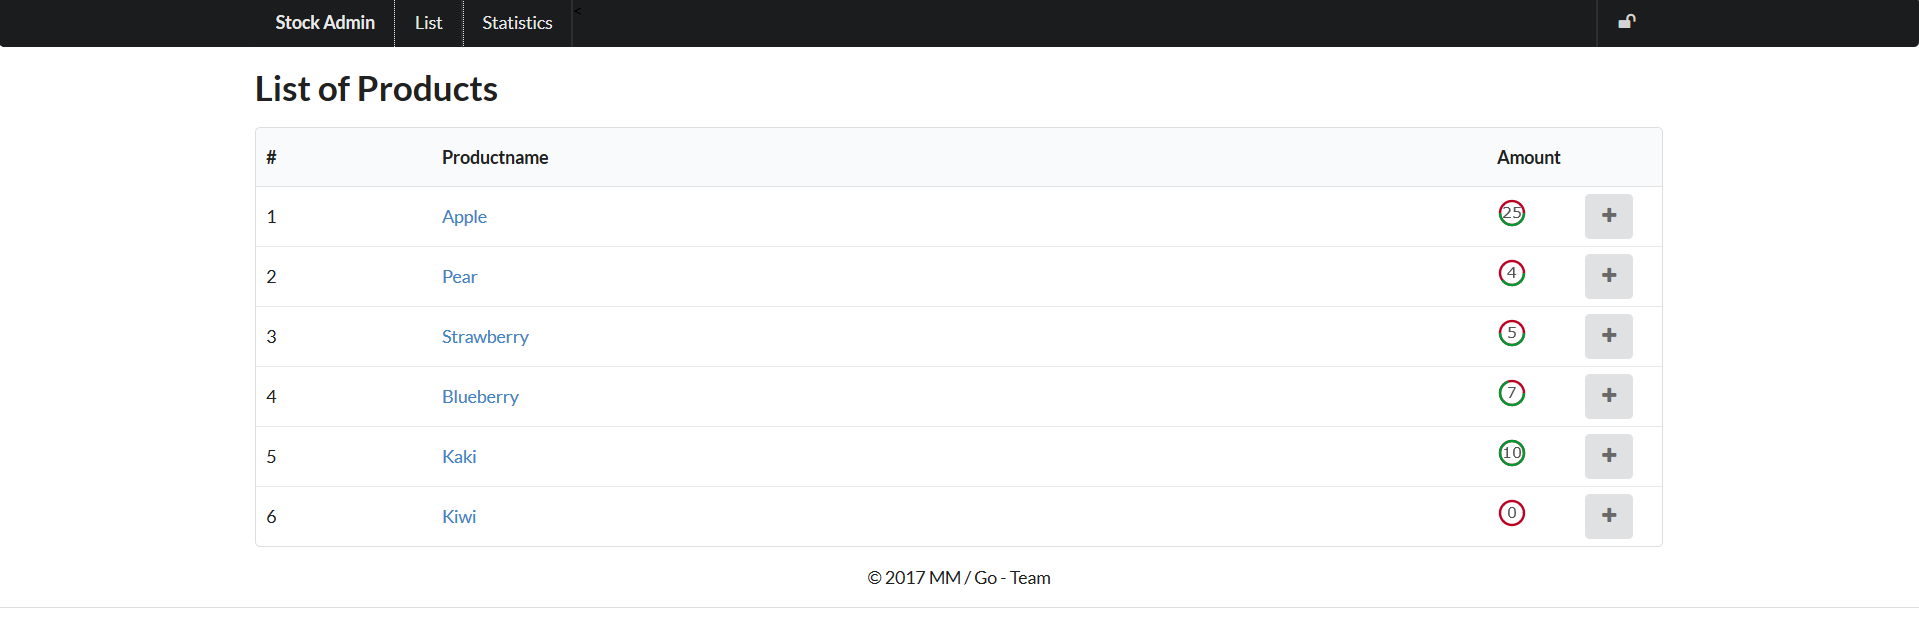
\includegraphics[width=0.75 \textwidth]{./pics/list.png}}
	\caption{Admin-Frontend -- List}
	\label{pic:Admin-Frontend -- List}
\end{figure}

\begin{figure}[H]
	\centering
	\frame{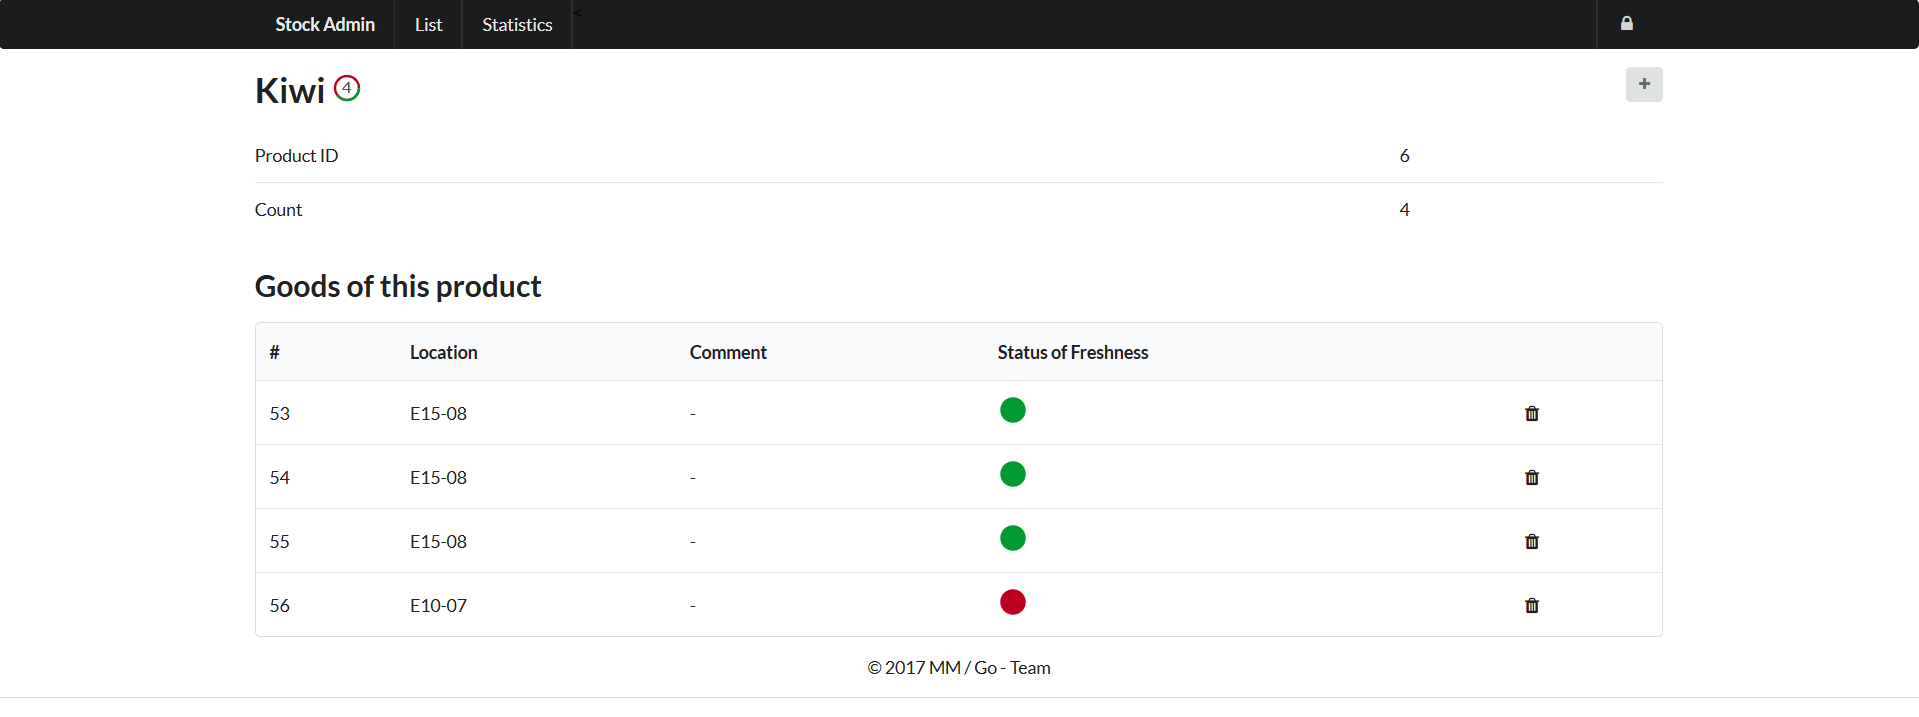
\includegraphics[width=0.75 \textwidth]{./pics/product.png}}
	\caption{Admin-Frontend -- Produktseite}
	\label{pic:Admin-Frontend -- Produktseite}
\end{figure}


\begin{figure}[H]
	\centering
	\frame{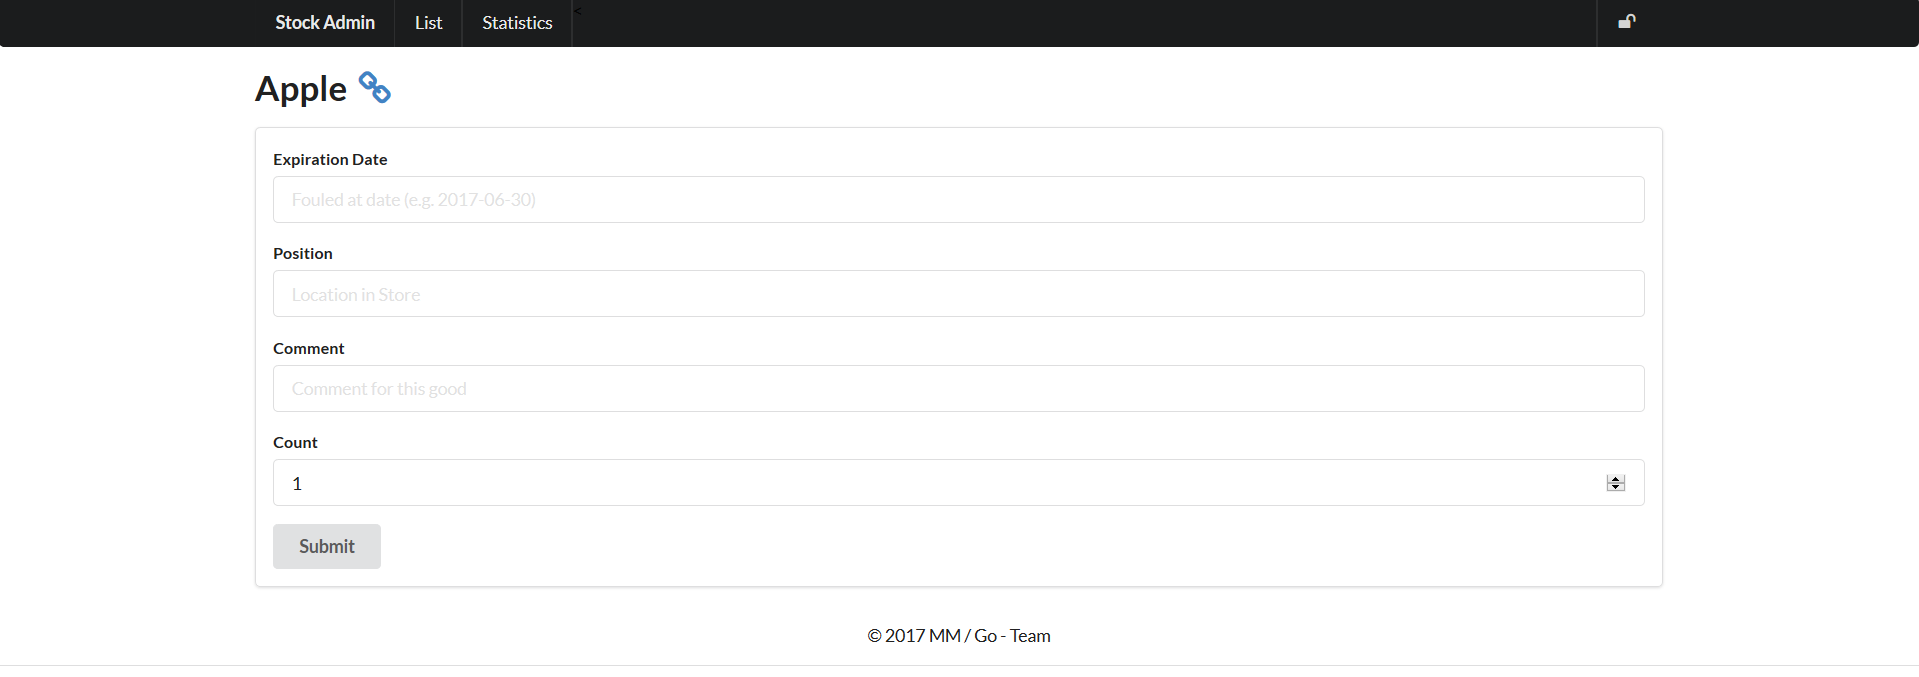
\includegraphics[width=0.75 \textwidth]{./pics/add.png}}
	\caption{Admin-Frontend -- Hinzufügen von Waren}
	\label{pic:Admin-Frontend -- Hinzufuegen von Waren}
\end{figure}


\newpage
\subsection{Application Layer}
\label{subsec: Application Layer}
Die Packages und Go-Files des Application Layers umfassen die Logik des Microservice Warenwirtschaft. Sie werden nachfolgend aufgelistet und kurz beschrieben.

\paragraph{cmd:} Go-File main.go, welches die Applikation letztendlich ausführt und alle Angaben zu den Config-Files der Applikation enthält

\paragraph{http:} Go-Files, die die Anwendungslogik (Funktionen) und die API-Routen beinhalten
	\begin{itemize}
	\item \texttt{bindapi.go}: Funktionen, die für das Binden der URL-Pfade notwendig sind
	\item \texttt{good.go}: Funktionen für das Hinzufügen von Waren zum Warenbestand und die Anzeige, ob eine Ware abgelaufen ist
	\item \texttt{good\_lock.go}: Funktionen für das Blockieren von Waren, die sich im Warenkorb befinden
		\item \texttt{good\_show.go}: Funktionen für die Auflistung und Zählung der vorhandenen Waren sowie die Feststellung ihrer Verfügbarkeit
	\item \texttt{good\_temp.go}: Hilfsfunktionen, die für die Darstellung des Warenbestandes als Ampel im Kunden-Frontend benötigt werden
	\item \texttt{status.go}: Funktion, die den Status des Microservice abfragt
	\end{itemize}


\paragraph{models:} Go-Files, die die zentralen Structs und zugehörige Hilfsfunktionen (hauptsächlich statischen Inhalt des Microservice) beinhalten
	\begin{itemize}
	\item \texttt{config.go}: Structs mit den Informationen zur Konfiguration des Webservers, der Datenbank und dem Cache-Management sowie Hilfsfunktionen zum Lesen von Config-Files
	\item \texttt{duration.go}: Structs und Hilfsfunktionen zur Definition eines Typs für Zeitangaben
	\item \texttt{good.go}: Structs und Hilfsfunktionen zur Darstellung von Waren, hier werden auch die geforderten Funktionalitäten wie das Blockieren von Waren umgesetzt
	\end{itemize}


\paragraph{runtime:} Go-Files mit weiteren Hilfsfunktionen
	\begin{itemize}
	\item \texttt{auth.go}: Hilfsfunktionen zur Prüfung, ob eine Berechtigung für den Zugriff vorliegt
	\item \texttt{cache\_worker.go}: Hilfsfunktionen für das Löschen und Anlegen von Cache-Workers
	\item \texttt{good\_fouled.go}: Hilfsfunktion, um abgelaufene Waren automatisch aus dem Warenbestand zu entfernen
	\item \texttt{good\_release.go}: Hilfsfunktionen zum Blockieren und Entsperren von Waren
	\item \texttt{productcache.go}: Hilfsfunktionen zum Anlegen eines Caches für Produkte
	\end{itemize}



\newpage
\paragraph{lib:} fasst die vier Packages \texttt{database}, \texttt{http}, \texttt{log} und \texttt{worker} zusammen

	\begin{itemize}
	\item \texttt{database}: Go-File \texttt{database.go} mit Funktionen für das Öffnen und Schließen der Datenbank
	\item \texttt{http}: Go-Files, die die Webserverlogik umgesetzten
		\begin{itemize}
		\item \texttt{io.go}: Funktionen zum Lesen und Schreiben von JSON aus beziehungsweise in HTTP-Pakete
		\item \texttt{permission.go}: Funktionen zur Prüfung der Berechtigung für den Zugriff
		\end{itemize}
	\item \texttt{log}: Go-File \texttt{log.go}, das den Logger startet und initiiert
	\item \texttt{worker}: Go-File \texttt{worker.go}, dass Funktionen für regelmäßige Aktivitäten bereitstellt. (z.B. das Entsperren von Waren nach einer vorgegeben Zeit)
	\end{itemize}


\subsection{Persistant Layer}
Der Persitant Layer umfasst beliebige SQL-Datenbanken, diesen Tabellen-Struktur beim starten automatisch angelegt. Die nachfolgende Abbildung \ref{pic:Datenbankmodell des Microservice} zeigt den grundsätzlichen Aufbau der Datenbank. Sie speichert den Warenbestand (stock). Zur Referenzierung wird vom Produkt die ID verwendet, die aus dem Produktkatalog bezogen und bei Anfrage in einem Cache zwischengespeichert werden. Vom Mircoservice werden nur die Waren (good) gespeichert und verwaltet, die eine ID, ein Ablaufdatum, eine Lagerposition und einen Kommentar besitzen. Dabei kann eine Ware nur zu einem Produkt gehören. Die Datenbank kann über die Konfigurationsdatei \texttt{config\_example.conf}, deren relevanter Ausschnitt nachfolgend dargestellt wird, flexibel angepasst werden. Zum Testen wurde eine SQL-Lite-Datenbank vorkonfiguriert, die im Cache gehalten wird.

\begin{figure}[H]
	\centering
	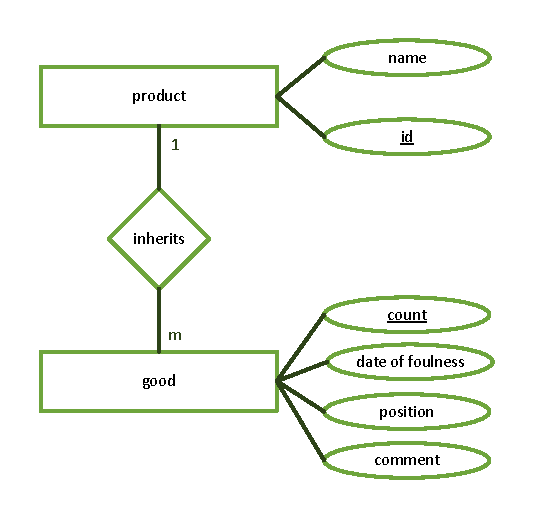
\includegraphics[width=0.40 \textwidth]{./pics/db.pdf}
	\caption{Datenbankmodell des Microservice}
	\label{pic:Datenbankmodell des Microservice}
\end{figure}


\begin{lstlisting}[caption=Datenbankeinstellungen in der Konfigurationsdatei]
[database]
type = "sqlite3"
# logging = true
connection = "file::memory:?mode=memory&cache=shared"
# For Master-Slave cluster
# read_connection = ""
\end{lstlisting}

\newpage
\subsection{Integrierte Tests}
\label{subsec: Integrierte Test}
Neben den bisherigen Packages, die bereits Whitebox-Tests umfassen, ist in dem Package \textbf{\texttt{test}} ein weiteres Go-File (\texttt{testrest.go}) enthalten. Dieses setzt einen Testumgebung um, bei dem auf Testdaten eines Produktkataloges zurückgegriffen wird. Mit Hilfe der integrierten Tests wird in der hier beschriebenen Version eine Code-Coverage von 100\% erreicht, das heißt jedes Stück Code wird mindestens einmal zur Ausführung gebracht.
Dies bedeutet nicht, dass dieser Mircoservice fehlerfrei ist, sondern lediglich das aus Entwickler-Sicht, alles getan wurde.

\subsection{Anpassung des Monolithen}
\label{subsec: Anpassung des Monolithen}
Damit der Microservice Warenwirtschaft durch den bestehenden Monolithen des Webshops Mosh genutzt werden kann, wurden hier die unter dem Anhang \ref{changes} aufgeführten Änderungen vorgenommen.
